\documentclass[11pt]{article}
\usepackage{a4wide}
\usepackage{fontspec}
\usepackage{xeCJK}

% Chinese Font Selection
% 宋体 and 楷体 are free fonts. Check out our GitHub repository to see the exact versions used.
\setCJKmainfont[ItalicFont = Kaiti SC, SlantedFont = STFangsong, BoldFont = Songti SC Bold]{Songti SC}
% Chinese Font Selection

\setCJKmainfont[
  Path = ../../fonts/Chinese/,
  ItalicFont = Kaiti.ttc,
  SlantedFont = STFangsong.ttf
]{Songti.ttc}

\setmainfont[ 
  Path = ../../fonts/CMUnicode/,
  Extension = .ttf,
  BoldFont = *-Bold,
  ItalicFont = *-Italic,
  BoldItalicFont = *-BoldItalic,
  SlantedFont = *-RomanSlanted,
  UprightFont = *-Roman
]{CMUSerif}
\setsansfont[
  Path = ../../fonts/CMUnicode/,
  Extension = .ttf,
  BoldFont = *-Bold,
  ItalicFont = *-Oblique,
  BoldItalicFont = *-BoldOblique,
  UprightFont = *
]{CMUSansSerif}
%\setmainfont[BoldFont = CMUSerif-Bold]{CMUSerif-Roman}
%\setsansfont{CMUSansSerif}

% "‘" & "’" might be recognized as CJK characters.
% Numbers are changed to make the date nature.
\normalspacedchars{‘’“”1234567890-—/̈}

\def \thistext{中文文本}
\def \nthIOL #1{#1国际语言学奥林匹克竞赛}
\def \thisth{第十届}
\def \thisland{斯洛文尼亚}
\def \thistown{卢布尔雅那}
\def \Julyname{七月}
\def \Auguname{八月}
\def \olydates #1#2#3#4#5{#5年#2#1日至#4#3日}
\def \leafword #1{答题纸 \##1}
\def \probword #1{题 \##1}
\def \probsing #1{#1 题目}
\def \probplur #1{#1 题目}
\def \respsing #1{#1 答案}
\def \solusing #1{#1 解答}
\def \soluplur #1{#1 解答}
\def \indicont{个人赛}
\def \teamcont{团队赛}
\def \Teamword{团队}
\def \pontword{分}
\def \regulats{解题规则}
\def \regulado{无需抄题}
\def \regulare{将每一道题的解答单独地写在的一张或几张纸上}
\def \regulami{在每张答题纸上标明题号、你的座位号和你的姓名}
\def \towarrant{否则你的工作可能会被错误地归类甚至遗失}
\def \regulaty{你的答案必须经过充分地论证}
\def \regulatz{即使一个全对的答案,没有解释,也会得低分}
\def \editorsz{编者}
\def \edinchef{主编}
\def \rulesmot{规则}
\def \answersp{答案}
\def \enquetex{问卷}
\def \enqueten{姓名}
\def \enquetep{座位号}
\def \enquetea{你做了哪些题目}
\def \enqueteb{你最喜欢哪道题}
\def \enquetec #1{你觉得哪道题#1}
\def \seemhard{最难}
\def \seemeasy{最简单}
\def \goodluck{祝你好运}
\def \quoted #1{“#1”}
\def \giveland #1{这里有#1个老挝语的国名}
\def \findland{辨认这些国家}
\def \guessond{猜测一下老挝语中国名的发音}
\def \givesent #1{这里有一些#1的句子}
\def \inBasque{巴斯克语}
\def \indiCent #1{#1的中部方言}
\def \giwordss #1{这里有一些#1的词和词组}
\def \ofRotuma{罗图马语}
\def \andtrans #1{及其#1翻译}
\def \chaotict{(乱序排列)}
\def \gyRotuma{这里有罗图马语的七个身体部位的名字}
\def \pasoreus{其中一句汉语对应两个巴斯克语句子}
\def \formahat #1{其中一句汉语有多种#1翻译}
\def \findtran{找出这个句子并给出其它可能的翻译}
\def \thremore #1{这里有另外三个#1的词}
\def \fordinto #1{翻译成#1}
\def \fordouta #1{将括号外的句子翻译成#1}
\def \tothislang{汉语}
\def \tolgEus{巴斯克语}
\def \tolgRtm{罗图马语}
\def \TheRtm{罗图马语}
\def \Thelg #1{#1}
\def \tolg #1{#1}
\def \lgUndu{温布-尤恩固语}
\def \lgTeop{蒂奥普语}
\def \Dyirbal{迪尔巴尔语}
\def \infamily #1#2{#1属于#2}
\def \toAustNs{南岛语系}
\def \toTNGfam{泛新几内亚语系}
\def \toPNyfam{帕马-恩永甘语系}
\def \spokenca #1#2{#2,大约#1人使用该语言}
\def \inPNG{在巴布亚新几内亚}
\def \inFiji{在斐济}
\def \spokNEQL{它是一个已经死亡的澳大利亚昆士兰州东北部的土著语言}
\def \corrcorr{找出正确的对应关系}
\def \writnums{写成数字}
\def \writeout #1{写成#1}
\def \canttran #1#2{仅仅使用上述材料,你不能肯定#2的#1翻译}
\def \whatposs #1{这些词的#1翻译理论上有哪些}
\def \stateopa #1{一位语言学家打算写出#1的语法规则}
\def \stateope{首先,她让她的信息提供人将这些独立的句子翻译成他们的母语}
\def \stateopi{这是她所得到的}
\def \stateopo #1{随后,这位语言学家记录了#1的自发性言语并往语法规则中加入了一些新信息}
\def \stateopu #1{这里给出了这些#1对话的一部分}
\def \stateopy{这些说出来的话的上文在括号中给出}
\def \bonaiana{这条鱼}
\def \bonaekae{这个包}
\def \bonaykae{\bonaekae}
\def \bonaover{这个椰子}
\def \paani #1#2{\iN{#1}吃了#2}
\def \teopdatg{你们听到了他}
\def \epaatara #1{看见了#1}
\def \teopdatu #1{看见了#1}
\def \teopdatf #1{我看见了#1}
\def \teopdatt{他看见了你们}
\def \who{主语}
\def \whotom{谁}
\def \what{什么}
\def \hee{给}
\def \enaaphee #1#2{我把#2给了#1}
\def \oteitomu{男人}
\def \beikoemu{孩子}
\def \heesoasi #1{把#1给了这个男孩}
\def \teopdati #1{把#1给了你们}
\def \teopdatm #1{我们把#1给了你}
\def \oraoraat{这个男巫}
\def \whom{谁}
\def \withwhat{用什么}
\def \tasu{打}
\def \teopdatc{我们打了那个孩子}
\def \teopdata{你打了我}
\def \teopdatj{我用石头打了你}
\def \teopdats #1{你用包打了#1}
\def \teopdatw{用椰子打了这个男孩}
\def \asun{杀}
\def \teopdato{我用它杀了他}
\def \litt{字面意义:}
\def \withim{用他}
\def \toraaram{用这个斧头}
\def \teopdatk #1{他们#1杀了这个女人}
\def \paaqasun #1#2{#2杀了#1}
\def \teopdate{杀了他}
\def \dao{称呼}
\def \whomcall{谁}
\def \whatcall{什么}
\def \teopdatl{我们称这个男孩为男巫}
\def \teopdatn{他称我为小孩}
\def \teopdaty{他们称这位男巫女人}
\def \thecerer{这位男巫}
\def \theboy{这个男孩}
\def \Theman{这个男人}
\def \men{男人们}
\def \Thewoman{这个女人}
\def \women{女人们}
\def \alltrest{所有其它东西}
\def \Why{为什么}
\def \didsocry #1{#1哭得这么厉害}
\def \offended #1{#1被冒犯了}
\def \teopdaqz{这个斧头是湿的}
\def \teopdaqv{这里没有留下任何食物}
\def \tabaqani{这些食物}
\def \tabaqany{\tabaqani}
\def \teopdaqu{接下来这个女人发生了什么}
\def \teopdaqx{这个包在哪里}
\def \mintzatu{与……谈了}
\def \mintzat{宾语}
\def \mintzaty #1#2{\iN{#1}与\iA{#2}谈了}
\def \hurbildu{与……接洽了}
\def \hurbild{宾语}
\def \hurbildy #1#2{\iN{#1}与\iA{#2}接洽了}
\def \ahaztu{忘了}
\def \ahazt{宾语}
\def \ahazty #1#2{\iN{#1}忘了\iA{#2}}
\def \lagundu{帮助了}
\def \lagund{宾语}
\def \lagundy #1#2{\iN{#1}帮助了\iA{#2}}
\def \ukitu{触摸了}
\def \ukit{宾语}
\def \ukity #1#2{\iN{#1}触摸了\iA{#2}}
\def \iN #1{\6#1(我,你,他,我们,你们,他们)}
\def \iA #1{\6#1(我,你,他,我们,你们,他们)}
\def \iD #1{#1}
\def \iJ #1{#1}
\def \dyirbalc{糖正在使这位健康的继母发胖}
\def \dyirbalh{酒正在使这个疲倦的医生入睡}
\def \dyirbale{这缕烟正在使这只蝎子感到疲倦}
\def \dyirbalf{这位被冒犯的父亲正在搬运酒}
\def \dyirbali{这只蜥蜴正在跟随这缕烟}
\def \dyirball{这个肥胖的医生正在推巨石}
\def \dyirbalj{这只蜻蜓正在搜寻刺痛树}
\def \dyirbald{这个疲倦的沙袋鼠正在搜寻小羽毛}
\def \dyirbaln{这只巨大的蚱蜢正在搜寻弯掉的矛}
\def \dyirbalo{这个安静的男孩正在看着这只疲倦的蜥蜴}
\def \dyirbalq{这只小沙袋鼠正在看着这只蜻蜓}
\def \dyirbals{这只睡着的袋貂正在无视着噪音}
\def \dyirbalp{这个总是被跟随的男人正在冒犯这位强壮的父亲}
\def \dyirbalr{这位一直被跟随的阿姨正在弯曲这根羽毛}
\def \dyirbalm{这位总是在推石头的继母正在看着这缕烟}
\def \dyirbalt{这只毛毛虫正在搜寻这个一直在搬石头的男人}
\def \dyirbalv{这只蜥蜴正在搜寻这个一直被推的石头}
\def \dyirbalu{这位总是被搜寻的父亲正在治疗这个女孩}
\def \dyirbala{酒正在使这个一直被责骂的男人感到疲倦}
\def \dyirbalw{这个总是责备医生的男人正在跟随这只沙袋鼠}
\def \dyirbalg{这条总是在搜寻蝎子的死蛇正在跟随这只袋貂}
\def \dyirbalb{这个强壮的男人正在责骂这位总是跟随死蛇的母亲}
\def \dyirbalk{这位总是被无视的母亲正在搬运糖}
\def \ngaymunga #1#2{总是在#1 #2}
\def \munga #1{总是被#1}
\def \bayimbam{毛虫}
\def \bayimbap{幼虫}
\def \auntword{阿姨}
\def \mugunanj{母亲的姐姐}
\def \muqgamot{噪音}
\def \defdeadd{死蛇是一种澳大利亚的毒蛇}
\def \defwalla{沙袋鼠是一种小动物,袋鼠的近亲}
\def \defpossu{袋貂是一种澳大利亚树栖的有袋目动物}
\def \defstree{刺痛树是一属有带刺茸毛的灌木和树, 其中一些对人类有害}
\def \thoughtE #1{一位语言学家认为上述#1句子中存在一处错误}
\def \nonerror{实际上,这里并没有错误}
\def \wheremis{你认为这位语言学家觉得哪里错了}
\def \theremis #1#2{这位语言学家认为样例#2中的#1是一处错误}
\def \babamyth #1#2{之所以这位语言学家感到怪异,是因为一种动物在#1的神话中被当作#2}
\def \oldwomen{老女人}
\def \oldwoman{老女人}
\def \bundinye{蚱蜢既不是女人,也不是一种危险动物,但使用了与两者相同的冠词}
\def \mustmyth #1{所以它一定是神话里的#1}
\def \animals{动物}
\def \dangerux #1{危险的#1和物体}
\def \whatanim{这是哪种动物}
\def \defcopra{干椰肉是干的椰子核}
\def \niu{干椰肉}
\def \niut #1{#1干椰肉}
\def \qolo{切}
\def \ququ{手臂/手}
\def \fau{年}
\def \aqoffau{年末}
\def \faega{词}
\def \huga{心}
\def \kia{脖子}
\def \hunkia{脖子底部}
\def \huni{低端}
\def \leva{头发}
\def \leavpiri{卷发}
\def \piri{卷曲(动词)}
\def \susu{胸}
\def \issusu{乳头}
\def \isu{鼻子}
\def \mafa{眼睛}
\def \maftiro{眼镜}
\def \tiro{玻璃}
\def \matmamas{冰}
\def \matiti{冷(名词)}
\def \mofa{垃圾}
\def \moafmofa{丢垃圾}
\def \poga{洞}
\def \poagpoga{布满洞的}
\def \pala{穿孔}
\def \nusutiro{窗户}
\def \nusura{门}
\def \pogi{夜晚}
\def \pulu{胶水}
\def \hafpraki{火山岩}
\def \hafu{岩石}
\def \hafhafu{布满岩石的}
\def \ruhuga{胃痛}
\def \toqa{英雄}
\def \kalkalu{圆的}
\def \kaluV{包围(动词)}
\def \kaluN{手镯}
\def \lala{深的}
\def \qelqele{浅的}
\def \huagqele{没有耐心的}
\def \huaglala{耐心的}
\def \huagtoqa{有勇气的}
\def \isqa{尖顶的}
\def \mafpogi{盲的}
\def \mamasa{固体}
\def \pulpulu{黏糊糊的}
\def \riamrima{锃亮的}
\def \qele{靠近(动词)}
\def \aqofi{使精疲力竭}
\def \faegay{说话(动词)}
\def \faeagqu{使用手语}
\def \huli{翻转(动词)}
\def \puhraki{使沸腾}
\def \rima{闪光}
\def \hulhafu{吹}
\def \hurrican{飓风}
\def \adjeverb #1{使#1}
\def \persnumb #1#2{第\ifcase #1\or 一\or 二\or 三\fi 人称#2}
\def \Sg{单数}
\def \Pl{复数}
\def \Perspron{人称代词}
\def \wordsord{语序是:}
\def \sestruct{这些句子的结构为}
\def \nounword{名词}
\def \adjectif{形容词}
\def \Verb{动词}
\def \Pred{predicate}
\def \Sb{主语}
\def \Ob{宾语}
\def \bis #1{另一个#1}
\def \attribut{修饰词}
\def \attribum{被修饰}
\def \ergatend{主语及其定语有后缀}
\def \worderNA{形容词跟在名词后面}
\def \incompoN{In a noun-noun compound}
\def \modihead{the second part modifies the first one}
\def \artnomen{每个名词前都有一个冠词}
\def \evelbona #1#2{如果是句子中第一个第三人称,则为#1,否则为#2}
\def \selepron #1#2{#1的代词的冠词,#2,也是以同样的方式决定的}
\def \topicfrt #1{在上文对话中提到的词将被移到句首,并使用冠词#1}
\def \pronoffe #1#2{如果因此,一个代词#1被移至动词的后面,它将会丢掉开头的#2}
\def \nounoffe #1#2{如果移动的#1是一个名词,它将保留它的冠词#2}
\def \temathes{当两个词构成一个短语时,第一个词的形态将发生如下变化}
\def \adjedoub{同样的情况发生在通过重复一个名词或动词构成一个形容词时}
\def \alsomean #1{也有#1的意思}
\def \hewhohas #1#2{拥有#1 #2的人}
\def \nounverb{产生的复合词可以为动词或者名词}
\def \simotend #1{如果这个词以#1结尾}
\def \byavowel{\vocal}
\def \byacsant{\const}
\def \vocal{元音}
\def \const{辅音}
\def \contains #1{有#1}
\def \twosylla{两个音节}
\def \trosylla{超过两个音节}
\def \samplart #1#2{是发音部位与#2相同的浊#1}
\def \stopcons{塞音}
\def \nasalcns{鼻音}
\def \wordlast{该词结尾最后一个音}
\def \velarnas{= 普通话 \word{杭} (\word{háng})里的\word{ng}}
\def \palatnas{= 普通话 \word{娘} (\word{niáng})里的\word{ni}}
\def \glotstop #1{#1是一个辅音(喉塞音)}
\def \oshiroko{= 普通话 \word{欧}}
\def \aeligatu #1{#1 $\approx$~\word{crack}里的\word a}
\def \oeumlaut{= 普通话 \word{约} 的元音}
\def \ueumlaut{= 普通话 \word{于} 的元音}
\def \longmark #1{标记~#1表示长元音}
\def \et #1{和#1}
\def \ett #1{且#1}
\def \ab{或}
\def \au{或}
\def \like{如}
\def \APname{Alexander Piperski}
\def \BIname{Boris Iomdin}
\def \DGname{Dmitry Gerasimov}
\def \IDname{戴谊凡}
\def \PSname{Pavel Sofroniev}
\def \XGname{Ksenia Gilyarova}
\def \LFname{Liudmila Fedorova}
\def \MKname{Maria Konoshenko}
\def \NZname{Natalya Zaika}
\def \SBname{Svetlana Burlak}
\def \MRname{Maria Rubinstein}
\def \ABname{Aleksandrs Berdičevskis}
\def \LPname{Aleksejs Peguševs}
\def \ASname{Artūrs Semeņuks}
\def \BLname{Bruno L’Astorina}
\def \HDname{Hugh Dobbs}
\def \GHname{Gabrijela Hladnik}
\def \RSname{Rosina Savisaar}
\def \JLname{李在揆}
\def \LMSname{刘闽晟}
\def \CQTname{曹起曈}
\def \edinames{\ABname, \SBname, \IDname(\edinchef), \HDname, \LFname, \DGname, \XGname, \GHname, \BIname, \BLname, \JLname, \LPname, \APname, \MRname, \RSname, \ASname, \PSname}
\def \whowroti{\LMSname,\CQTname,\IDname}
\def \idLand{印度尼西亚}
\def \kpLand{朝鲜}
\def \ngLand{尼日利亚}
\def \afLand{阿富汗}
\def \thLand{泰国}
\def \fiLand{芬兰}
\def \skLand{斯洛伐克}
\def \lvLand{拉脱维亚}
\def \cnLand{中国}
\def \ghLand{加纳}
\def \iqLand{伊拉克}
\def \ieLand{爱尔兰}
\def \yeLand{也门}
\def \pkLand{巴基斯坦}
\def \loLand{老挝}
\def \dzLand{阿尔及利亚}
\def \isLand{冰岛}
\def \npLand{尼泊尔}
\def \dkLand{丹麦}
\def \snLand{塞内加尔}
\def \inLand{印度}
\def \azLand{阿塞拜疆}
\def \noLand{挪威}
\def \gtLand{危地马拉}
\def \cmLand{喀麦隆}
\def \aeLand{阿联酋}
\def \ilLand{以色列}
\def \coLand{哥伦比亚}
\def \soLand{索马里}
\def \krLand{韩国}
\def \nlhLand{荷兰}
\def \veLand{委内瑞拉}
\def \srLand{塞尔维亚}
\def \zaLand{南非}
\def \alLand{阿尔巴尼亚}
\def \cuLand{古巴}
\def \peLand{迷路}
\def \joLand{约旦}
\def \luLand{卢森堡}
\def \vnLand{越南}
\def \saLand{沙特阿拉伯}
\def \nzLand{新西兰}
\def \itLand{意大利}
\def \amLand{亚美尼亚}
\def \syLand{叙利亚}
\def \irLand{伊朗}
\def \bgLand{保加利亚}
\def \uzLand{乌兹别克斯坦}
\def \geLand{格鲁吉亚}
\def \trLand{土耳其}
\def \maLand{摩洛哥}
\def \caLand{加拿大}
\def \usLand{美国}
\def \keLand{肯尼亚}
\def \ptLand{葡萄牙}
\def \boLand{玻利维亚}
\def \mdLand{摩尔多瓦}
\def \nlLand{尼德兰}
% Run RemoveSpace to get IOL10.nospace.tex
%\addtolength{\oddsidemargin}{-.875in}
%\addtolength{\evensidemargin}{-.875in}
%\addtolength{\topmargin}{-.525in}
%\addtolength{\textwidth}{1.75in}
%\addtolength{\textheight}{1.4in}
%\usepackage{colortbl}
\usepackage{graphicx}

\newenvironment{assgts}{%
\renewcommand \labelenumi {\bfseries \zagrad {\alph {enumi}}}%
\renewcommand \labelenumii {\arabic {enumii}.}%
\begin{enumerate}}{\end{enumerate}}

\newcommand \by [1]{%
  \unskip\nobreak\hfil\penalty50
  \hbox{}\nobreak\hfill{\hbox{\qquad\itshape #1}}\par}
%\newcommand \book[1]{{\slshape #1\/}}
\newcommand \bord [1]{{\bfseries\itshape\selectfont #1\/}}
\newcommand \word [1]{{\itshape #1\/}}
\newcommand \ipaword [1]{[\ipa{#1}]}

% IPA Input
% XeLaTeX has built-in Unicode support, which means IPA input becomes a simple font selection problem.
\newfontfamily \IPAFont{CMUSerif-Roman}
\newcommand \ipa [1]{\bgroup\IPAFont #1\egroup}
\newcommand \bipa [1]{\bgroup\bfseries\IPAFont #1\egroup}
% The following is old LaTeX code.
% \newcommand \ipa [1]{\bgroup\fontencoding{T3}\selectfont\SetUnicodeOption{tipa}#1\egroup}
% \newcommand \bipa [1]{\bgroup\fontencoding{T3}\bfseries\selectfont\SetUnicodeOption{tipa}#1\egroup}
% IPA Input

\let \super \textsuperscript
\newcommand \synt [1]{\L{\textsf{#1}}}
\newcommand \tallstrut {\vrule height 9pt depth 0pt width 0pt}
\newcommand \deepstrut {\vrule height 0pt depth 2pt width 0pt}
\newcommand \placehold {\fbox{\fbox{\quad} \fbox{\quad} \fbox{\quad}}}
\def \hh {\textsuperscript h}
%\let \visiblespace \textvisiblespace
\newcommand \latehta [1]{\quoted{#1\space}}
\newlength\halftext
\halftext=\textwidth \advance \halftext by-50pt \divide \halftext by2
\newcommand \NB {{\ooalign{\hfil\raise.2ex\hbox{\bfseries!}\hfil\crcr\Large$\bigtriangleup$}}}
\ifx \upcase \undefined \newcommand \upcase [1]{\MakeUppercase {#1}}\fi
\newcommand \Upcase {\expandafter \upcase }
\newcommand \Uppcase {\expandafter \expandafter \expandafter \Upcase }
\ifx \zagrat \undefined \newcommand \zagrat [1]{\zagrad{#1.}}\fi
%\newcommand \upsens [2]{\MakeUppercase {#1#2}}
%\newcommand \thead {\expandafter \upsens }
%\let \thead \relax
\mathchardef\nga="223A

\def \6#1(#2,#3,#4,#5,#6,#7){\ifcase #1\or #2\or #3\or #4\or #5\or #6\or #7\fi}

\makeatletter
\def \ps@somestyle {
\let\@oddfoot\@empty
\def\@oddhead{\ifx \N \relax
\textsl {\small \begin{tabular}[t]{@{}l}\nthIOL {\thisth}\ \zagrad{\N{2012}}.\\ \chapname \end{tabular}}\hfill \thepage
\else \thepage \hfill
\textsl {\small \begin{tabular}[t]{r@{}}\R{\nthIOL {\thisth}\ \zagrad{\N{2012}}.}\\ \R{\chapname} \end{tabular}}
\fi }}
%\def \procherk {\hrulefill}
\def \procherk {\leaders \hbox {:}\hfill \kern\z@}
\makeatother

\newcounter {exx}[section]
\newcounter {ex:bundiny}
\ifx \N \undefined
  \let \N \relax
  \let \R \relax
  \let \L \relax
  \newcommand \zagrad [1]{(#1)}
  \def \lr {l}\def \bimapp {rll}
  \newcommand \biline [2]{\addtocounter{exx}{1}\arabic{exx}. & #1. & #2}
  \newcommand \ciline [3]{\addtocounter{exx}{1}\arabic{exx}. & \multicolumn{2}{l}{(#1?)} \\ & #3 & #2.}
  \newcommand \bidyir [2]{\addtocounter{exx}{1}\arabic{exx}. & \bipa{#1.} \\& #2.}
  \newcommand \biriyd [2]{\addtocounter{exx}{1}\arabic{exx}. & #1. \\& \bipa{#2.}}
%  \newcommand \squoted [1]{`#1'}
  \newcommand \squoted [1]{‘#1’}
\else
  \renewcommand \bord [1]{\L{\bfseries\itshape\selectfont #1\/}}
  \renewcommand \bipa [1]{\L{\bgroup\fontencoding{T3}\bfseries\selectfont\SetUnicodeOption{tipa}#1\egroup}}
  \newcommand \zagrad [1]{)#1(}
  \def \lr {r}\def \bimapp {lrl}
  \newcommand \biline [2]{#2 & \R{#1.} & \addtocounter{exx}{1}.\arabic{exx}}
  \newcommand \ciline [3]{&\hfill \R{)#1?(} & \addtocounter{exx}{1}.\arabic{exx}\\ \R{#2.} & #3}
  \newcommand \bidyir [2]{\bipa{#1.} & \addtocounter{exx}{1}.\arabic{exx}\\\hfill \R{#2.}}
  \newcommand \biriyd [2]{\hfill \R{#1.} & \addtocounter{exx}{1}.\arabic{exx}\\\bipa{#2.}}
  \newcommand \squoted [1]{\L{'}#1\L{`}}
\fi
\ifx \zagrad \undefined \fi
\ifx \postpar \undefined \newcommand \postpar {.}\fi
\newcommand \paaS [2]{\bord{#1 paa #2.}}

\newcommand \georow [3]{#1. & \R{#3} & \ipa{[#2]}}

\def \problem {\stepcounter {section}\paragraph{\probword \thesection\ \zagrad{\N{20} \pontword}\postpar }}
\def \solution {\stepcounter {section}\paragraph{\probword \thesection \postpar }}

\newcommand \makepart [1]{\newpage
\thispagestyle{empty}
  \begin{center}%
  {\LARGE \nthIOL {\thisth} \par }
  \vskip 1em{\Large
  \thistown\ \zagrad {\thisland}, \olydates {30}{\Julyname}{3}{\Auguname}{2012}
  \par }
%  \vskip 1em{\begin{tabular}[t]{c}\Large
%  \thistown\ (\thisland), \olydates {30}{\Julyname}{3}{\Auguname}{2012}
%  \end{tabular}\par }
  \vskip 1em{\large #1}\end{center}\par \vskip .5em
  \def \chapname {#1}\setcounter {section}0\setcounter {page}1}

\newcount \uuq
\newcount \uur
\newcount \uux
\newcount \uuy
\newcommand \nuu [1]{\ifcase #1\or telu\or talu\or yepoko\fi}
\newcommand \tuu [1]{\uux=#1\advance\uux by-2
  \ifnum 18<\uux tokapu yepoko \advance\uux by-18
  \else \ifnum 12<\uux tokapu talu \advance\uux by-12
  \else \ifnum 6<\uux tokapu \advance\uux by-6
  \fi\fi\fi
  \ifcase \uux\or rurepo\or malapu\or supu\or tokapu\or alapu\or polangipu\or 9\fi}
\newcommand \uu [1]{%
  \ifnum #1<4\nuu {#1}\else
  \uur=#1
  \ifnum 48=\uur tokapu talu\else \ifnum 72=\uur tokapu yepoko\else
    \uuy=#1\divide \uuy by4\uuq=\uuy
    \multiply \uuy by4\advance \uur by-\uuy
    \ifnum0=\uur
      \tuu{\uuq}%
    \else
      \advance \uuq by1\tuu{\uuq}nga \nuu {\uur}%
    \fi
  \fi\fi\fi}
\newcommand \borduu [1]{\bord {\uu {#1}}}
\newcommand \duu [1]{$#1$ & \borduu {#1}}

\begin{document}
\ifx\enumLat\undefined\else\enumLat\fi

\thispagestyle{empty}
\makepart{\probplur {\indicont}}

\pagestyle{somestyle}

%\centerline{\textbf{\regulats}}
%
\regulado. \regulare. \regulami. \towarrant.

\regulaty. \regulatz.\bigskip

\hrule

\problem \givesent {\indiCent {\Dyirbal}}\andtrans {\tothislang}:\medskip \\
%
\begin{tabular}{ll}
\bidyir{bayi yaɽa ŋunɟaymuŋa baŋgu gurugugu biŋgunman}{\dyirbala}\\
\bidyir{balan yabu bimabanɟalŋaymuŋa baŋgul yaɽaŋgu guliŋgu ŋunɟaɲu}{\dyirbalb}\\
\bidyir{balan waymin bambun baŋgu ɟugaŋgu ɟamiman}{\dyirbalc}\\
\bidyir{bala yila wura baŋgul bargandu biŋgundu guniɲu}{\dyirbald}\\
\bidyir{balan malayigara baŋgu garandu biŋgunman}{\dyirbale}\\
\bidyir{bala gurugu baŋgul ŋumaŋgu munduŋgu dimbaɲu}{\dyirbalf}\\
\bidyir{bayi midin baŋgun bimaŋgu malayigaraguninaymuŋagu banɟan}{\dyirbalg}\\
\bidyir{bayi gubimbulu biŋgun baŋgu gurugugu ɟagunman}{\dyirbalh}\\
\bidyir{bala garan baŋgul biɲɟiriɲɟu banɟan}{\dyirbali}\\
\bidyir{balan duŋan baŋgul yiriɲɟilagu guniɲu}{\dyirbalj}\\
\bidyir{bala ɟuga baŋgun yabuŋgu ŋaɟilmuŋagu dimbaɲu}{\dyirbalk}\\
\bidyir{bala diban ɟagiɲ baŋgul gubimbulugu ɟamiŋgu bilmban}{\dyirball}\\
\bidyir{bala garan baŋgun waymindu dibanbilmbalŋaymuŋagu buɽan}{\dyirbalm}\\
\bidyir{balan baŋgay waɽu baŋgun bundiɲɟu ɟagiɲɟu guniɲu}{\dyirbaln}\setcounter {ex:bundiny}{\value {exx}}\\
\bidyir{bayi biɲɟiriɲ biŋgun baŋgul ɲalŋgaŋgu mugurugu buɽan}{\dyirbalo}\\
\bidyir{bayi ŋuma guli baŋgul yaɽaŋgu banɟalmuŋagu munduman}{\dyirbalp}\\
\end{tabular}
%
\begin{assgts}
\item \thoughtE {\Dyirbal}. \nonerror. \babamyth {\Dyirbal}{\quoted {\oldwomen}}. \whatanim? \wheremis?
\item \fordinto {\tothislang}:
\begin{enumerate}\setcounter{enumii}{\value{exx}}
\item\bipa{balan ɲalŋga baŋgul ŋumaŋgu guniymuŋagu bambunman.}
\item\bipa{bala diban bilmbalmuŋa baŋgul biɲɟiriɲɟu guniɲu.}
\item\bipa{bayi bargan baŋgul yaɽaŋgu gubimbuluŋunɟanaymuŋagu banɟan.}
\setcounter{exx}{\value{enumii}}
\end{enumerate}
\item \thremore {\Dyirbal}:
%
\begin{quote}
\bipa{bayimbam} — \bayimbap\if0\bayimbam \else, \bayimbam\fi; \\
\bipa{mugunanɟa} — \auntword\ \zagrad{\mugunanj}; \\
\bipa{muŋga} — \muqgamot.
\end{quote}
%
\fordinto {\tolg {\Dyirbal}}:
\begin{enumerate}\setcounter{enumii}{\value{exx}}
\item \dyirbalq.
\item \dyirbalr.
\item \dyirbals.
\item \dyirbalt.
\end{enumerate}
\end{assgts}
%
\NB \quad \infamily {\Thelg {\Dyirbal}}{\toPNyfam}; \spokNEQL.

\bipa{ŋ} \velarnas.

\bipa{ɲ} \palatnas;
\bipa{ɟ} \samplart {\stopcons\ \zagrad{\like\ \bipa d}}{\bipa{ɲ}}.

\defdeadd. \defwalla. \defpossu. \defstree.
%\defigrog.
%
\by{—\ASname}

\newpage

\problem \mbox{}\medskip\\
%
\begin{tabular}{l|l}
& \R{\lgUndu} \\\hline
\duu{10}\\
\duu{15}\\
\duu{20}\\
\duu{21}\\
\duu{27}\\
\duu{30}\\
\end{tabular}\hfill
\fbox{\L{\borduu 1 < \borduu 3}}\hfill
\begin{tabular}{l|l}
& \R{\lgUndu} \\\hline
\duu{35}\\
\duu{40}\\
\duu{48}\\
\duu{50}\\
\duu{69}\\
\duu{79}\\
\duu{97}\\
\end{tabular}
%
\begin{assgts}
\item \writnums:
\begin{tabular}[t]{l}
\borduu {56},\\
\borduu {57},\\
\borduu {86},\\
\borduu {101}.
\end{tabular}
%
\item \writeout {\lgUndu}: $13$; $66$; $72$; $76$; $95$.
\end{assgts}
%
\NB \quad \infamily {\Thelg{\lgUndu}}{\toTNGfam}. \spokenca{34\,200}{\inPNG}.
%
\by{—\XGname\deepstrut}

\bigskip

\problem \givesent {\inBasque}\andtrans {\tothislang}\chaotict. \pasoreus:
%
\begin{center}
\bord{ahaztu ditut,
ahaztu zaizkit,
ahaztu zaizu,
hurbildu natzaizue,
hurbildu zait,
lagundu ditugu,
lagundu dituzu,
lagundu dute,
lagundu nauzue,
mintzatu natzaizu,
mintzatu gatzaizkizue,
mintzatu zaizkigu,
ukitu ditugu,
ukitu naute}\medskip

\ahazty 23,
\mintzaty 64,
\hurbildy 15,
\mintzaty 12,
\lagundy 46,
\lagundy 51,
\hurbildy 31,
\ukity 46,
\ukity 61,
\lagundy 26,
\lagundy 63,
\mintzaty 45,
\ahazty 16
\end{center}
%
\begin{assgts}
\item \corrcorr.
\item \fordinto {\tolgEus}: \ukity 21, \hurbildy 61.
\item \fordinto {\tothislang}: \bord{lagundu dut}, \bord{hurbildu gatzaizkizu}.
\item \formahat {\tolgEus}. \findtran.
\end{assgts}
%
\by{—\NZname}

\newpage

\problem
\stateopa {\lgTeop}.
\stateope.
\stateopi:\medskip\\
%
\begin{tabular}{\bimapp}
\biline {\teopdata}{\paaS{Ean}{tasu anaa}}\\
\biline {\paani 3{\bonaiana}}{\paaS{Eove}{ani bona iana}}\\
\biline {\teopdatc}{\paaS{Enam}{tasu a beiko}}\\
\biline {\Theman\epaatara {\bonaykae}}{\paaS{A otei}{tara bona kae}}\\
\biline {\Upcase \theboy\teopdate}{\paaS{A visoasi}{asun bona}}\\
\biline {\teopdatf {\tabaqany}}{\paaS{Enaa}{tara a taba’ani}}\\
\biline {\teopdatg}{\paaS{Eam}{baitono e}}\\
\biline {\enaaphee {\oteitomu}{\bonaover}}{\paaS{Enaa}{hee a otei bona overe}}\\
\biline {\Thewoman\teopdati {\tabaqani}}{\paaS{A moon}{hee ameam bona taba’ani}}\\
\biline {\teopdatj}{\paaS{Enaa}{tasu vuan a vasu}}\\
\biline {\teopdatk {\toraaram}}{\paaS{Eori}{asun bona moon bona toraara}}\\
\biline {\teopdatl}{\paaS{Enam}{dao a visoasi bona oraoraa}}\\
\end{tabular}
%
\begin{assgts}
\item \fordinto {\tothislang}:
\begin{enumerate}\setcounter{enumii}{\value{exx}}
\item\paaS{Eam}{ani a overe}
\item\paaS{Ean}{tasu a oraoraa bona kae}
\item\paaS{Eove}{tara ameam}
\setcounter{exx}{\value{enumii}}
\end{enumerate}
\item \fordinto {\tolg {\lgTeop}}:
\begin{enumerate}\setcounter{enumii}{\value{exx}}
\item \teopdatm {\tabaqani}.
\item \teopdatn.
\item \teopdato\ \zagrad{\emph{\litt}\ \withim}.
\item \Upcase \thecerer\heesoasi {\bonaiana}.
\setcounter{exx}{\value{enumii}}
\end{enumerate}
\end{assgts}
%
\stateopo {\lgTeop}.
\stateopu {\lgTeop}\andtrans {\tothislang}.
\stateopy.\medskip\\
%
\begin{tabular}{rll}
\ciline {\teopdaqu}{\Thewoman\teopdatu {\oraoraat}}{\paaS{A moon}{tara bona oraoraa}}\\
\ciline {\Why\teopdaqv}{\paani 4{\tabaqani}}{\paaS{A taba’ani}{ani nam}}\\
\ciline {\Why\didsocry {\theboy}}{\Theman\teopdatw}{\paaS{A visoasi}{tasu a otei bona overe}}\\
\ciline {\teopdaqx}{\enaaphee {\beikoemu}{\bonaekae}}{\paaS{A kae}{hee naa a beiko}}\\
\end{tabular}
%
\begin{assgts}\setcounter{enumi}{2}
\item \fordouta {\tolg {\lgTeop}}:
\begin{enumerate}\setcounter{enumii}{\value{exx}}
\item \zagrad {\Why\offended {\thecerer}?}\ \teopdaty.
\item \zagrad {\Why\teopdaqz?}\ \Upcase \theboy\paaqasun {\bonaiana}{\toraaram}.
\end{enumerate}
\end{assgts}
%
\NB \quad \infamily {\Thelg{\lgTeop}}{\toAustNs}. \spokenca{5\,000}{\inPNG}.
%
\by{—\MKname}

\newpage

\problem \giwordss {\ofRotuma}\andtrans {\tothislang}:\medskip \\
%
\begin{tabular}{l\ifx \N \relax l\else r\fi}
\bord{‘el‘ele} & \R{\qelqele} \\
\bord{‘ele} & \R{\qele} \\
\bord{‘olo} & \R{\qolo} \\
\bord{a‘öf fau} & \R{\aqoffau} \\
%\bord{a‘öf susu} & \R{\aqofsusu} \\
\bord{fäeag ‘u‘u} & \R{\faeagqu} \\
%\bord{fäeag toko} & \R{\faeagtoko} \\
\bord{fau} & \R{\fau} \\
\bord{hạfhạfu} & \R{\hafhafu} \\
\bord{huag ‘el‘ele} & \R{\huagqele} \\
\bord{huag to‘a} & \R{\huagtoqa} \\
\bord{hül hạfu} & \R{\hulhafu\ \zagrad{\hurrican}} \\
\bord{hün kia} & \R{\hunkia} \\
\bord{huli} & \R{\huli} \\
\bord{huni} & \R{\huni} \\
\bord{is ‘ā} & \R{\isqa} \\
\bord{is susu} & \R{\issusu} \\
\bord{lala} & \R{\lala} \\
\bord{maf tiro} & \R{\maftiro} \\
\end{tabular}\hfill
\begin{tabular}{l\ifx \N \relax l\else r\fi}
\bord{mamasa} & \R{\mamasa} \\
\bord{mạtiti} & \R{\matiti} \\
\bord{mạtit mamasa} & \R{\matmamas} \\
\bord{moafmofa} & \R{\moafmofa} \\
\bord{niu} & \R{\niu} \\
\bord{nu‘suar tiro} & \R{\nusutiro} \\
\bord{nu‘sura} & \R{\nusura} \\
\bord{pala} & \R{\pala} \\
\bord{piri} & \R{\piri} \\
\bord{poagpoga = palpala} & \R{\poagpoga} \\
\bord{pogi} & \R{\pogi} \\
\bord{puhrạki} & \R{\puhraki} \\
\bord{pulu} & \R{\pulu} \\
%\bord{rạhu} & \R{\rahu} \\
\bord{kạlu} & \R{\kaluN; \kaluV} \\
\bord{riamrima} & \R{\riamrima} \\
\bord{rū huga} & \R{\ruhuga} \\
\bord{to‘a} & \R{\toqa} \\
%\bord{toko} & \R{\toko} \\
\end{tabular}
%
\begin{assgts}
\item \gyRotuma\andtrans {\tothislang}\chaotict. \corrcorr:\smallskip

\centerline{\bord{‘u‘u, isu, kia, leva, mafa, susu, huga}}
\centerline{\R{\susu, \mafa, \ququ, \leva, \huga, \kia, \isu}}
\item \fordinto {\tothislang}:\smallskip

\centerline{\bord{tiro, poga} \R{\zagrad{\nounword}}\bord{, huag lala, hạf puhrạki, maf pogi = maf pala.}}
\item \fordinto {\tolgRtm}:\smallskip

\centerline{\R{%
%\rahrahu;
\kalkalu;
\niut {\qolo};
\leavpiri;
\pulpulu;
\rima;
\mofa.}}
\item \canttran{\tolgRtm}{\squoted{\faega} \et {\squoted{\aqofi}}}. \whatposs {\tolgRtm}?
\end{assgts}
%
\NB \quad \infamily {\TheRtm}{\toAustNs}. \spokenca {9000}{\inFiji}.

\glotstop {\bord{‘}};
\bord{ạ} \oshiroko;
\aeligatu {\bord{ä}};
\bord{ö} \oeumlaut;
\bord{ü} \ueumlaut.
\longmark {\quoted{\L{\bfseries¯}}}.

\defcopra.
%
\by{—\BIname, \APname}

\vfill
%\hline

\begin{center}
\textbf{\editorsz:} \edinames.\medskip

\textbf{\thistext:} \whowroti.\medskip

\large \goodluck!
\end{center}

\makepart{\soluplur {\indicont}}
%\thispagestyle{empty}
\pagestyle{somestyle}
%
\solution \wordsord\ \fbox{\synt{OSV}}
\zagrad{\synt O: \Ob, \synt S: \Sb, \synt V: \Verb},
\fbox{\synt{NA}}
\zagrad{\synt N: \nounword, \synt A: \adjectif}.

\synt{A $\to$ V} \zagrad{\squoted{\adjeverb {\synt A}}}: \L{\synt A\bipa{-man}}.

\synt{V $\to$ A}:
\begin{tabular}[t]{|l|l|l|}\hline
\synt V & \R{\squoted{\munga {\synt V}}} & \R{\squoted{\ngaymunga {\synt V}{\synt N}}} \\\hline
\bipa{-n} & \bipa{-l-muŋa} & \synt N-\dots\bipa{-l-ŋay-muŋa} \\
\bipa{-ɲu} & \bipa{-y-muŋa} & \synt N-\dots\bipa{-nay-muŋa} \\\hline
\end{tabular}\medskip

\artnomen:\medskip \\
%
\begin{tabular}{|l|l|\lr|}\hline
\synt O & \synt S & \\\hline
\bipa{balan} & \bipa{baŋgun} & \R{\women, \dangerux {\animals}} \\
\bipa{bayi} & \bipa{baŋgul} & \R{\men, \animals} \\
\bipa{bala} & \bipa{baŋgu} & \R{\alltrest} \\\hline
\end{tabular}
\medskip \\

\ergatend
\begin{itemize}
\item \bipa{-ŋgu}, \simotend {\byavowel}\et {\contains {\twosylla}};
\item \bipa{-gu}, \simotend {\byavowel}\et {\contains {\trosylla}};
\item \L{\textbf{-Du}}, \simotend {\byacsant};
\L{\textbf D} \samplart {\stopcons}{\wordlast}.
\end{itemize}
%
\begin{assgts}
\item \bundinye, \mustmyth {\quoted {\oldwoman}}. \theremis {\bipa {baŋgun bundiɲɟu}}{\zagrad{\arabic {ex:bundiny}}}.
\setcounter{exx}{16}
\item \begin{tabular}[t]{ll}
\bidyir{balan ɲalŋga baŋgul ŋumaŋgu guniymuŋagu bambunman}{\dyirbalu}\\
\bidyir{bala diban bilmbalmuŋa baŋgul biɲɟiriɲɟu guniɲu}{\dyirbalv}\\
\bidyir{bayi bargan baŋgul yaɽaŋgu gubimbuluŋunɟanaymuŋagu banɟan}{\dyirbalw}\\
\end{tabular}
\item \begin{tabular}[t]{ll}
\biriyd{\dyirbalq}{bayi yiriɲɟila baŋgul bargandu wuraŋgu buɽan}\\
\biriyd{\dyirbalr}{bala yila baŋgun mugunanɟagu banɟalmuŋagu waɽuman}\\
\biriyd{\dyirbals}{bala muŋga baŋgul midindu ɟagundu ŋaɟin}\\
\biriyd{\dyirbalt}{bayi yaɽa dibandimbanaymuŋa baŋgul bayimbambu guniɲu}\\
\end{tabular}
\end{assgts}

\solution \mbox{}

\begin{tabular}{r|l}
& \R{\lgUndu} \\\hline
\duu{1}\\
\duu{2}\\
\duu{3}\\
\duu{12}\\
\duu{16}\\
\duu{20}\\
\duu{24}\\
\duu{28}\\
\duu{32}\\
\end{tabular}\hfill
\begin{tabular}{l|l}
& \R{\lgUndu} \\\hline
$24$ & \borduu {24}\\
$48=24\times 2$ & \borduu {48}\\
$72=24\times 3$ & \borduu {72}\\
$\alpha \nga \beta := (\alpha-4)+\beta$, & $\alpha\mbox{\bord{-nga}}\ \beta$\\
\quad $\alpha \in \{12,16,20,24,28,32\},$\\
\quad $\beta \in \{1,2,3\}$\\
$\gamma + \delta$, & $\gamma\ \delta$\\
\quad $\gamma = 24k, k \in \{1,2,3\}$,\\
\quad $9\le \delta\le 32, \delta \ne 24$\\
\end{tabular}
%
\begin{assgts}
\item \begin{tabular}[t]{l}
\borduu {56} = $24+32 = 56$,\\
\borduu {57} = $24\times 2+12 \nga 3 = 57$,\\
\borduu {86} = $24\times 3+16 \nga 2 = 86$,\\
\borduu {101} = $24\times 3+32 \nga 1 = 101$.
\end{tabular}
%
\item \begin{tabular}[t]{l}
$13 = 16\nga 1$ = \borduu{13},\\
$66 = 24\times 2+20\nga 2$ = \borduu{66},\\
$72 = 24\times 3$ = \borduu{72},\\
$76 = 24\times 2+28$ = \borduu{76},\\
$95 = 24\times 3+24\nga 3$ = \borduu{95}.
\end{tabular}
\end{assgts}

\solution \mbox{}\smallskip \\
%
\begin{tabular}{|l|l|l|l|l|l|l|}\hline
 & \R{\persnumb1{\Sg}} & \R{\persnumb1{\Pl}}
 & \R{\persnumb2{\Sg}} & \R{\persnumb2{\Pl}}
 & \R{\persnumb3{\Sg}} & \R{\persnumb3{\Pl}}\\\hline
\L{A} & \bord{nau-} & & & & \bord{du-} & \bord{ditu-}\\\hline
\L{B} & \bord{natzai-} & \bord{gatzaizki-} & & & \bord{zai-} & \bord{zaizki-}\\\hline
\L{Z} &\hfill \bord{-t} &\hfill \bord{-gu} &\hfill \bord{-zu} &\hfill \bord{-zue} & &\hfill \bord{-te}\\\hline
%\L{A} & \bord{n-au-} & & & & \bord{d-u-} & \bord{d-it-u-}\\\hline
%\L{B} & \bord{n-at-zai-} & \bord{g-at-zai-zki-} & & & \bord{zai-} & \bord{zai-zki-}\\\hline
%\L{Z} &\hfill \bord{-t} &\hfill \bord{-gu} &\hfill \bord{-zu} &\hfill \bord{-zue} & &\hfill \bord{-te}\\\hline
\end{tabular}
\\
\begin{tabular}{|l|*{4}{\lr|}}\hline
& \L{A} & \L{B} & \L{Z} & \\\hline
\bord{ahaztu} & \multicolumn{2}{c|}{— \R{\ahazt} —} & \R{\who} & \R{\ahaztu} \\\hline
\bord{hurbildu} && \R{\who} & \R{\hurbild} & \R{\hurbildu} \\\hline
\bord{lagundu} & \R{\lagund} && \R{\who} & \R{\lagundu} \\\hline
\bord{mintzatu} && \R{\who} & \R{\mintzat} & \R{\mintzatu} \\\hline
\bord{ukitu} & \R{\ukit} && \R{\who} & \R{\ukitu} \\\hline
\end{tabular}
%
\begin{assgts}
\item \mbox{}\\
\centerline{\begin{tabular}{l\lr}
$\left.\begin{array}{@{}l}\mbox{\bord{ahaztu ditut}} \\\mbox{\bord{ahaztu zaizkit}}\end{array}\right\}$ & \R{\ahazty 16} \\
\bord{ahaztu zaizu} & \R{\ahazty 23} \\
\bord{hurbildu natzaizue} & \R{\hurbildy 15} \\
\bord{hurbildu zait} & \R{\hurbildy 31} \\
\bord{lagundu ditugu} & \R{\lagundy 46} \\
\bord{lagundu dituzu} & \R{\lagundy 26} \\
\end{tabular}\hfill
\begin{tabular}{\ifx \N \relax ll\else lr\fi}
\bord{lagundu dute} & \R{\lagundy 63} \\
\bord{lagundu nauzue} & \R{\lagundy 51} \\
\bord{mintzatu natzaizu} & \R{\mintzaty 12} \\
\bord{mintzatu gatzaizkizue} & \R{\mintzaty 45} \\
\bord{mintzatu zaizkigu} & \R{\mintzaty 64} \\
\bord{ukitu ditugu} & \R{\ukity 46} \\
\bord{ukitu naute} & \R{\ukity 61} \\
\end{tabular}}
\item \ukity 21\ — \bord{ukitu nauzu}, \hurbildy 61\ — \bord{hurbildu zaizkit}.
\item \bord{lagundu dut} — \lagundy 13, \bord{hurbildu gatzaizkizu} — \hurbildy 42.
\item \ahazty 23\ \zagrad{\bord{ahaztu zaizu}} — \bord{ahaztu duzu}.
\end{assgts}

\solution \sestruct: \fbox{\L{\textsf{S} \bord{paa} \textsf{V O [O${}^{'}$]}}}
\zagrad{\synt S: \Sb, \synt V: \Verb, \synt O: \Ob, \synt{O${}^{'}$}: \bis {\Ob}}.\medskip\\
%
\begin{tabular}{|l|\lr|\lr|\lr|}\hline
& \R{\hee} & \R{\dao} & \R{\tasu, \asun} \\\hline
\synt O & \R{\whotom} & \R{\whomcall} & \R{\whom} \\
\synt{O${}^{'}$} & \R{\what} & \R{\whatcall} & \R{\withwhat} \\\hline
\end{tabular}\medskip

\artnomen, \evelbona {\bord{a}}{\bord{bona}}.
\selepron {\persnumb3{\Sg}}{{\bord{e}} \au\ {\bord{bona}}}.

\Perspron:\medskip\\
%
\begin{tabular}{|\lr|l|l|l|l|l|l|}\hline
 & \R{\persnumb1{\Sg}} & \R{\persnumb1{\Pl}}
 & \R{\persnumb2{\Sg}} & \R{\persnumb2{\Pl}}
 & \R{\persnumb3{\Sg}} & \R{\persnumb3{\Pl}}\\\hline
\synt S & \bord{enaa} & \bord{enam} & \bord{ean} & \bord{eam} & \bord{eove} & \bord{eori}\\\hline
\synt O, \synt{O${}^{'}$} & \bord{anaa} & & \bord{vuan} & \bord{ameam} & \bord e, \bord{bona} &\\\hline
\end{tabular}
%
\begin{assgts}
\item
\begin{enumerate}\setcounter{enumii}{12}
\item\paaS{Eam}{ani a overe} — \paani 5{\bonaover}.
\item\paaS{Ean}{tasu a oraoraa bona kae} — \teopdats {\oraoraat}.
\item\paaS{Eove}{tara ameam} — \teopdatt.
\setcounter{exx}{\value{enumii}}
\end{enumerate}
\item
\begin{enumerate}\setcounter{enumii}{\value{exx}}
\item \teopdatm {\tabaqani}. — \paaS{Enam}{hee vuan a taba’ani}
\item \teopdatn. — \paaS{Eove}{dao anaa bona beiko}
\item \teopdato. — \paaS{Enaa}{asun e bona}
\item \Upcase \thecerer\heesoasi {\bonaiana}. — \paaS{A oraoraa}{hee bona visoasi bona iana}
\setcounter{exx}{\value{enumii}}
\end{enumerate}
\end{assgts}
%
\newsavebox{\topics}
\newlength{\topicswide}\newlength{\topicsleft}
\savebox{\topics}{\fbox{\begin{tabular}[t]{r@{ \bord{paa} \textsf V }l@{ $\to$ }r@{ \bord{paa} \textsf V }l}
\synt{\underline S} & \L{\textsf{O [O${}^{'}$]}} & \L{\textsf{\underline S}} & \L{\textsf{O [O${}^{'}$]}} \\
\synt S & \synt{\underline O [O${}^{'}$]} & \synt{\underline O} & \synt{S [O${}^{'}$]} \\
\synt S & \synt{O \underline{O${}^{'}$}} & \synt{\underline {O${}^{'}$}} & \synt{S O} \\
\end{tabular}}}
\settowidth{\topicswide}{\usebox{\topics}}
\topicsleft=\textwidth \advance\topicsleft by-10pt\advance\topicsleft by-\topicswide
\parbox{\topicsleft}{\topicfrt {\bord{a}}.
\pronoffe {\Sb}{\bord{e-}}.
\nounoffe {\Sb}{\bord a}.}\hfill
\parbox{\topicswide}{\usebox{\topics}}
%
\begin{assgts}\setcounter{enumi}{2}
\item
\begin{enumerate}\setcounter{enumii}{\value{exx}}
\item \zagrad {\Why\offended {\thecerer}?}\ \teopdaty.\\— \paaS{A oraoraa}{dao ori bona moon}
\item \zagrad {\Why\teopdaqz?}\ \Upcase \theboy\paaqasun {\bonaiana}{\toraaram}.\\
— \paaS{A toraara}{asun a visoasi bona iana}
\end{enumerate}
\end{assgts}

\newpage

%\solution \twoforms:\medskip \\
\solution \temathes:\medskip \\
%
\begin{tabular}{|l@{ $\to$ }l}
%\longform & \kortform \\\hline
\synt{-VCV} & \synt{-VC} \\
\synt{-VC}\bord u & \synt{-VC} \\
\synt{-VC}\bord i & \synt{-\"VC} \\
\synt{-VC}\bord a & \synt{-V}\bord a\synt C \\
\end{tabular}
\smallskip\
%
\zagrad{\synt V: \vocal, \synt C: \const}.

%\inphrase.
\adjedoub: \L{\bord{‘ele} + \bord{‘ele} $\to$ \bord{‘el‘ele}} \squoted{\qele\ $\times$ 2 = \qelqele}.

\wordsord
\begin{itemize}
\item \fbox{\synt{N$_1$ N$_2$}} \zagrad{\synt{N$_1$}: \attribum, \synt{N$_2$}: \attribut};
\item \fbox{\synt{N A}} \zagrad{\alsomean \squoted {\hewhohas {\synt A}{\synt N}}:
\bord{huag ‘el‘ele} \squoted{\huga\ + \qelqele\ = \huagqele}};
\item \fbox{\synt{V O}} \zagrad{\nounverb:
\bord{a‘öf fau} \squoted{\aqofi\ + \fau\ = \aqoffau},
\bord{hül hạfu} \squoted{\huli\ + \hafu\ = \hulhafu\ \zagrad{\hurrican}}}.
\end{itemize}

\begin{assgts}
\item
\bord{‘u‘u} — \ququ,
\bord{isu} — \isu,
\bord{kia} — \kia,
\bord{leva} — \leva,
\bord{mafa} — \mafa,
\bord{susu} — \susu,
\bord{huga} — \huga.
\item
\bord{tiro} — \tiro,\\
\bord{poga} — \poga,\\
\bord{huag lala} — \huaglala,\\
\bord{hạf puhrạki} — \hafpraki,\\
\bord{maf pogi = maf pala} — \mafpogi.
\item
%\rahrahu\ — \bord{rạhrạhu};
\kalkalu\ — \bord{kạlkạlu};
\niut {\qolo} — \bord{‘ol niu};
\leavpiri\ — \bord{leav pirpiri};
\pulpulu\ — \bord{pulpulu};
\rima\ — \bord{rima};
\mofa\ — \bord{mofa}.
\item
\begin{itemize}
\item \faega: \bord{fäega} \zagrad{\au\ \bord{fäeaga, fäeagu}}.
\item \aqofi: \bord{a‘ofi} \zagrad{\au\ \bord{a‘öfi, a‘öfö, a‘öfu, a‘öfü, a‘ofü}}.
\end{itemize}
\end{assgts}

\makepart {\enquetex}
\enqueten:\vskip 1in

\enquetep:\vskip 1in

\enquetea?\vskip 1in

\enqueteb?\vskip 1in

\enquetec {\seemhard}?\vskip 1in

\enquetec {\seemeasy}?

\makepart{\probsing {\teamcont}}
%\thispagestyle{empty}
\pagestyle{somestyle}

\giveland {\N{57}}:

% geo57Lao.pdf
% Things changed because of XeLaTeX
% It just works and I don't know the reason.
% Good luck!
\L{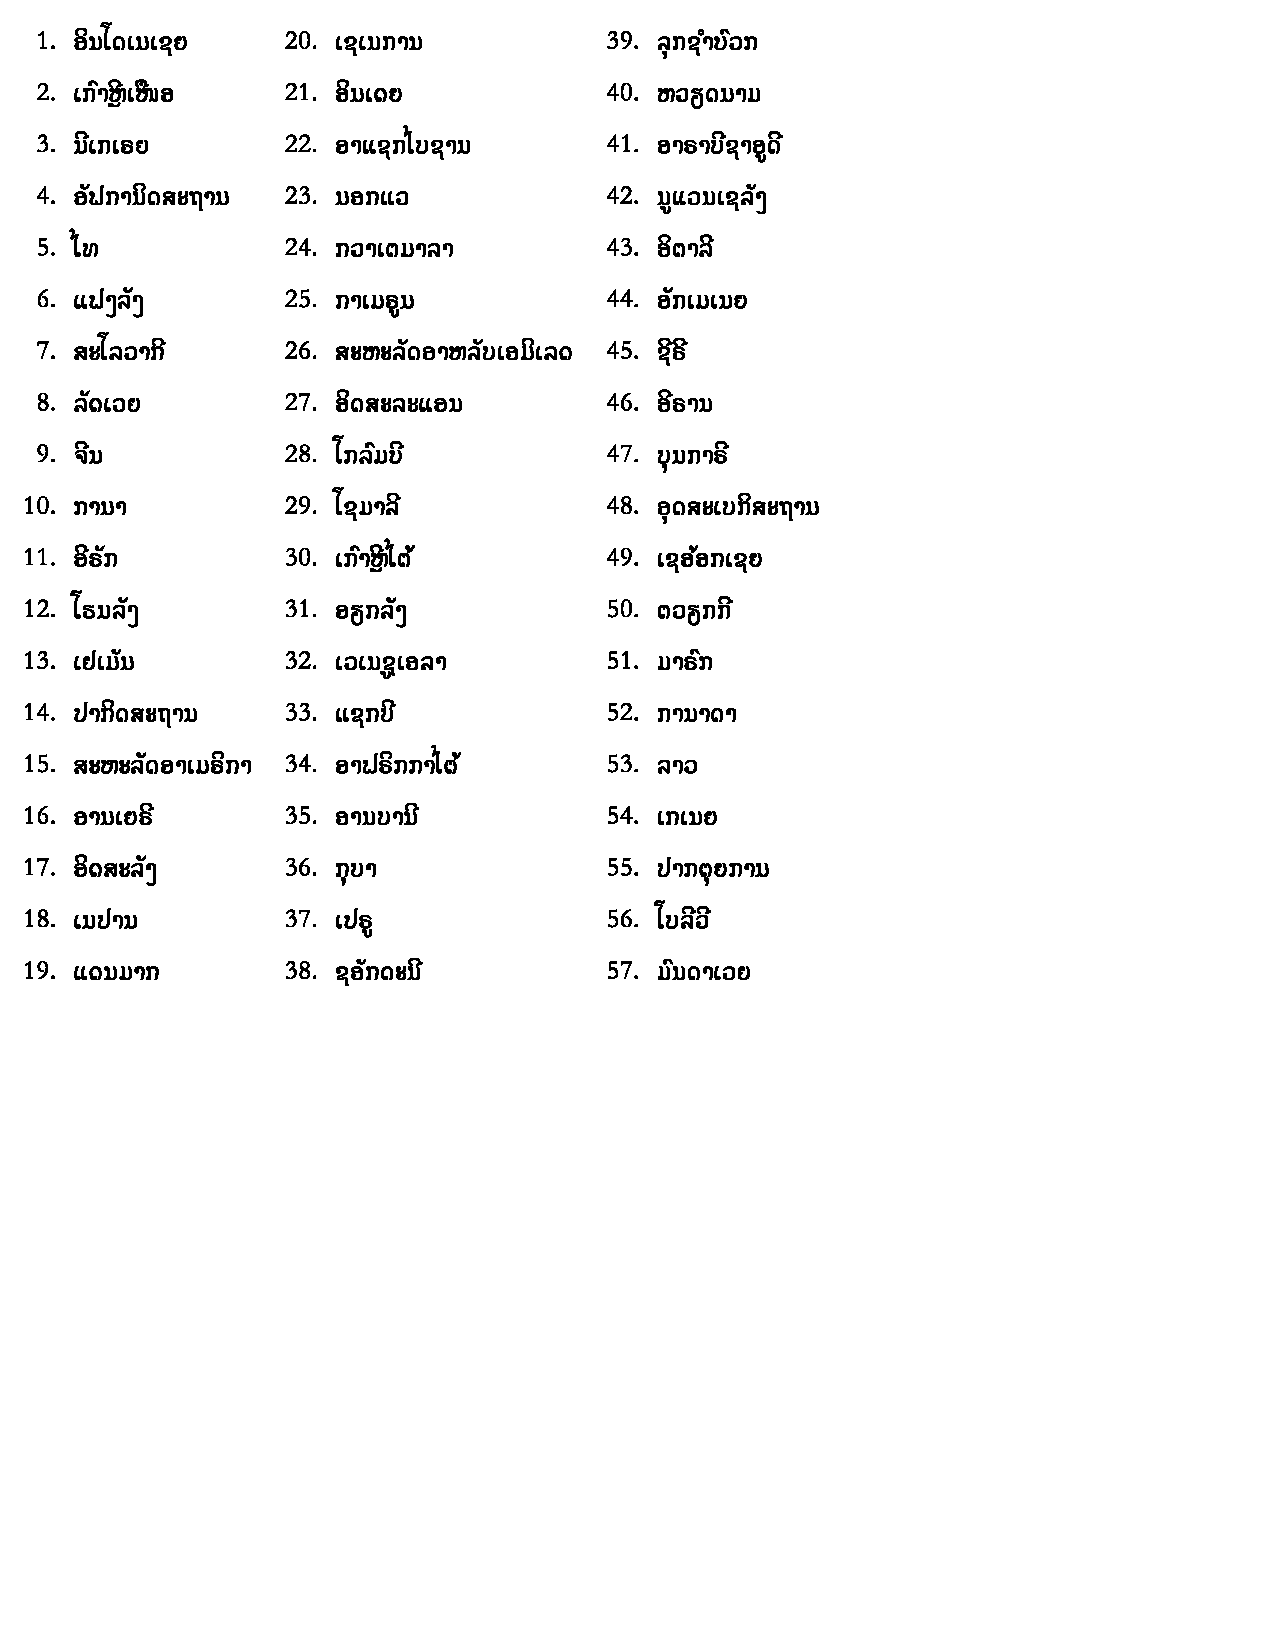
\includegraphics[trim = 0 320 320 0]{geo57Lao.pdf}}
%\L{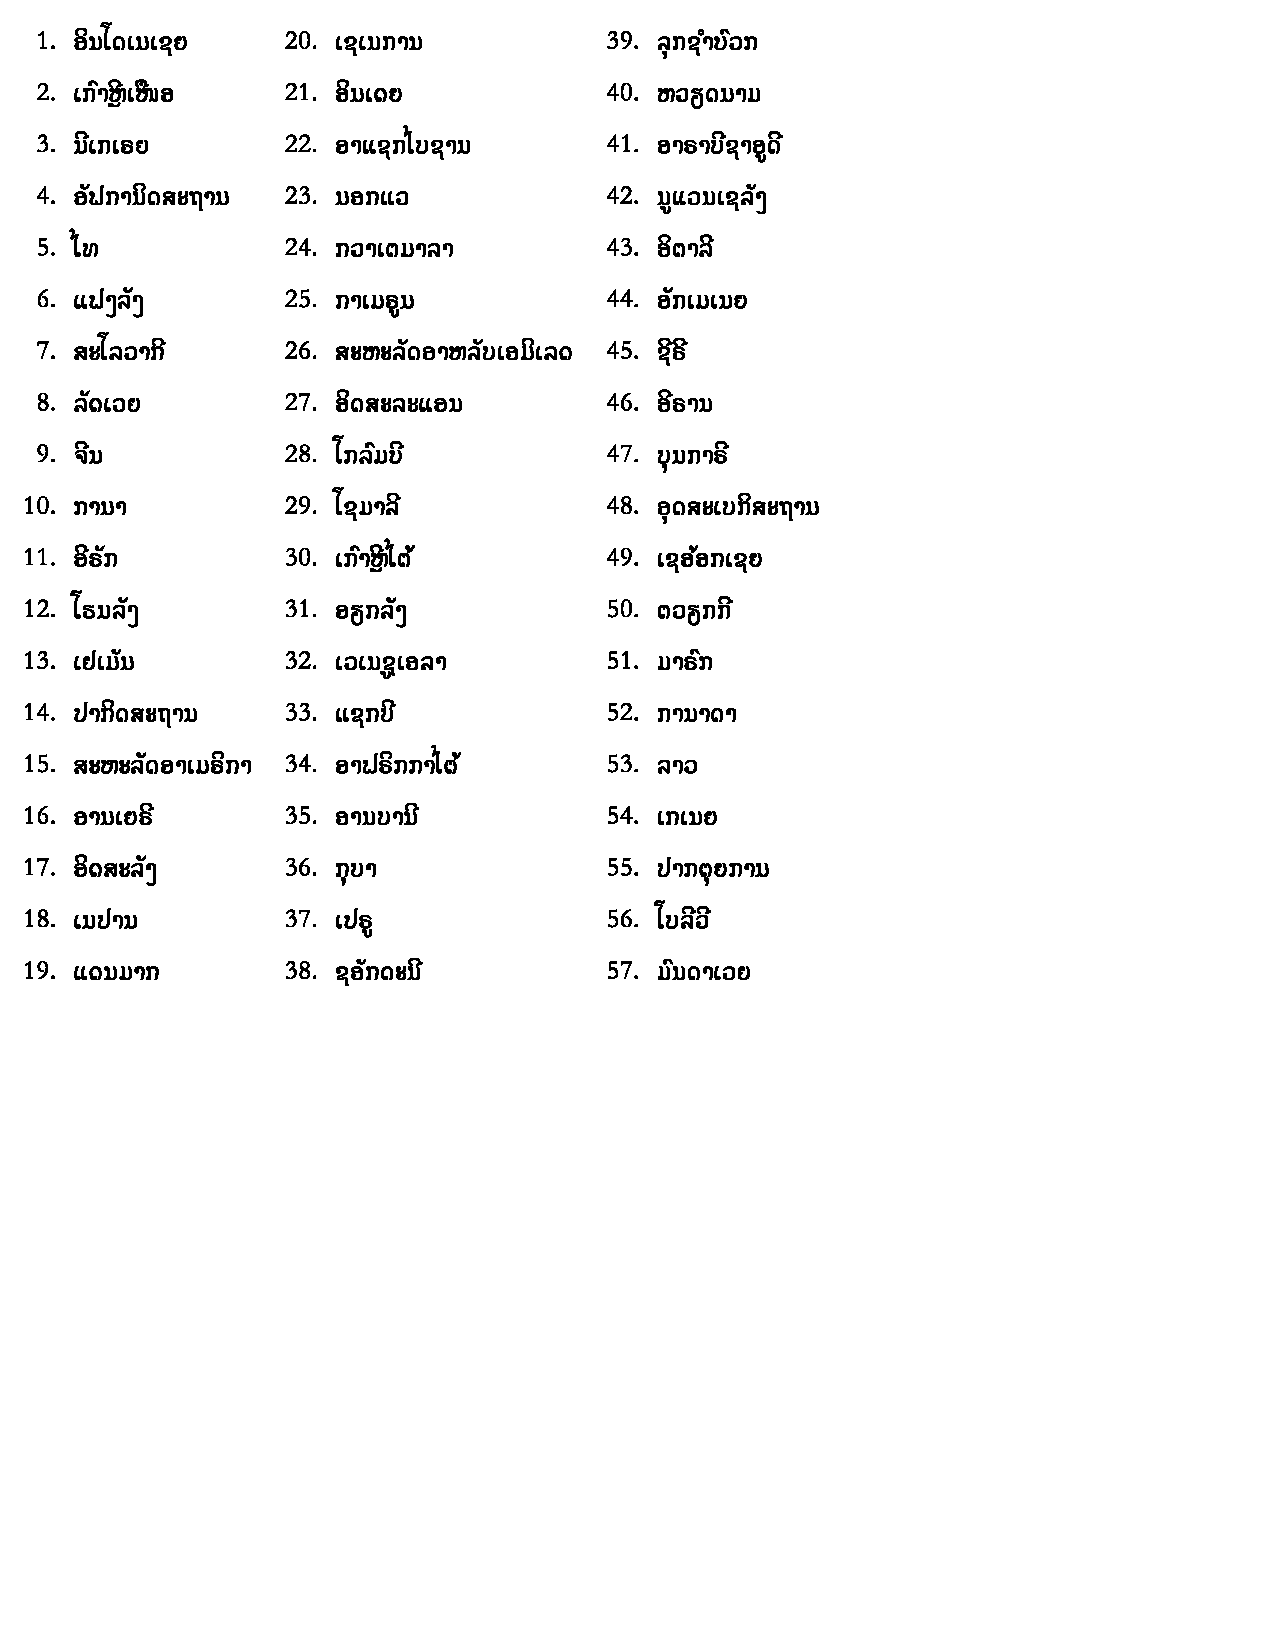
\includegraphics[bb = 0 320 500 800]{geo57Lao.pdf}}
% geo57Lao.pdf

%
\begin{assgts}
\item \findland.
\item \guessond.
\end{assgts}
%
\by{—\BIname}

\makepart{\respsing {\teamcont}}
%\makepart{\solusing {\teamcont}}
%\thispagestyle{empty}
\pagestyle{somestyle}

\centerline{\begin{tabular}{r\lr l}
\georow{1}{indōnēsiya}{\idLand}\\
\georow{2}{kaw{\super h}ḷī {\super h}n\={ʉ}a}{\kpLand}\\
\georow{3}{nīkēliya}{\ngLand}\\
\georow{4}{âfkānitsatʰān}{\afLand}\\
\georow{5}{tʰai}{\thLand}\\
\georow{6}{fǣṅlâṅ}{\fiLand}\\
\georow{7}{salōvākī}{\skLand}\\
\georow{8}{lâtviya}{\lvLand}\\
\georow{9}{čīn}{\cnLand}\\
\georow{10}{kānā}{\ghLand}\\
\georow{11}{īlâk}{\iqLand}\\
\georow{12}{hōnlâṅ}{\nlhLand\ \zagrad{\nlLand}}\\
\georow{13}{yēmen}{\yeLand}\\
\georow{14}{pākitsatʰān}{\pkLand}\\
\georow{15}{sahalât āmēlikā}{\usLand}\\
\georow{16}{ānñēlī}{\dzLand}\\
\georow{17}{itsalâṅ}{\isLand}\\
\georow{18}{nēpān}{\npLand}\\
\georow{19}{dǣnmāk}{\dkLand}\\
\georow{20}{sēnēkān}{\snLand}\\
\georow{21}{indiya}{\inLand}\\
\georow{22}{āsækbaisân}{\azLand}\\
\georow{23}{n\={ɔ}kvǣ}{\noLand}\\
\georow{24}{kwātēmālā}{\gtLand}\\
\georow{25}{kāmēlūn}{\cmLand}\\
\georow{26}{sahalât ā{\super h}lâp ēmilēt}{\aeLand}\\
\georow{27}{itsala'ǣn}{\ilLand}\\
\georow{28}{kōlômbī}{\coLand}\\
\georow{29}{sōmālī}{\soLand}\\
\end{tabular}
\begin{tabular}{r\lr l}
\georow{30}{kaw{\super h}ḷī tái}{\krLand}\\
\georow{31}{aẏklâṅ}{\ieLand}\\
\georow{32}{vēnēsū'ēlā}{\veLand}\\
\georow{33}{sǣkbī}{\srLand}\\
\georow{34}{āflikkā tái}{\zaLand}\\
\georow{35}{ānbānī}{\alLand}\\
\georow{36}{kubā}{\cuLand}\\
\georow{37}{pēlū}{\peLand}\\
\georow{38}{sɔkdanī}{\joLand}\\
\georow{39}{luksāṃbuak}{\luLand}\\
\georow{40}{{\super h}wẏatnām}{\vnLand}\\
\georow{41}{ālābī sā'ūdī}{\saLand}\\
\georow{42}{nūvǣn ṣēlâṅ}{\nzLand}\\
\georow{43}{itālī}{\itLand}\\
\georow{44}{âkmēniya}{\amLand}\\
\georow{45}{sīlī}{\syLand}\\
\georow{46}{īlān}{\irLand}\\
\georow{47}{bunkālī}{\bgLand}\\
\georow{48}{utsabēkisatʰān}{\uzLand}\\
\georow{49}{sē'óksiya}{\geLand}\\
\georow{50}{twaẏkkī}{\trLand}\\
\georow{51}{mālôk}{\maLand}\\
\georow{52}{kānādā}{\caLand}\\
\georow{53}{lāw}{\loLand}\\
\georow{54}{kēniya}{\keLand}\\
\georow{55}{pāktuykān}{\ptLand}\\
\georow{56}{bōlīvī}{\boLand}\\
\georow{57}{môndāviya}{\mdLand}\\
\end{tabular}}

\end{document}

